% Chapter 12 (English edition) -- ED-15: does the triangular lattice minimise the harmonic zero-point energy? (numerical counterexample)
% Translated from papers/discovery_journal_2026/chapters/c12.tex. Figure: code/fig12.py.
\chapter[Testing before proving]{Testing before proving: a natural idea that does not hold up}

\reference{Preprint of 25 October 2026, published on 26 October 2026. doi:10.5281/zenodo.23653833}

\section*{The idea in one picture}

Marbles that push each other away, lying on a table, settle into triangles, like the cells of a
honeycomb. For a wide family of repulsions, this arrangement is the cheapest when the marbles
are motionless. For the bell-shaped repulsion, this is an old result from the literature; for
the whole family, the proof published in 2026 was produced by an AI and has not yet been read by
specialists.

But in quantum physics nothing is completely still: even at absolute zero, every particle
trembles, and this trembling costs an energy called the ``zero-point energy''. The natural idea,
labelled QU-1 in the project, was that the champion at rest stays champion once this trembling
is counted. It was written down in advance, with an estimate (six chances in ten that it
survives) and a rule: we would only try to prove it if it first passed a numerical test. It did
not pass.

\begin{analogie}
Connect the marbles with invisible springs. At rest, we count the tension stored in the springs:
that is where the triangle wins. The trembling, by contrast, is like a note that each way of
vibrating hums non-stop; the zero-point energy is the sum of all these notes. If we deform the
arrangement a little, some notes go up and others go down. But the pitch of a note varies like
the \emph{square root} of the stiffness: gains and losses no longer cancel as they do for the
tension, and for some bells it is the low notes that win out.
\emph{Where the picture stops:} there are no springs and no sound; a ``note'' is a wave running
through the whole lattice, not the vibration of one isolated spring, and the calculation
compares frozen arrangements, it follows no motion.
\end{analogie}

\section*{What was done}

The test covered twelve repulsions from the family: bells of five widths, two screened
repulsions of the kind found in plasmas, two repulsions between electron--hole pairs in layered
materials, and three inverse powers of the distance. For several hundred lattice shapes, a
program computes all the vibrations, discards the unstable lattices (those where a vibration
runs away), and then adds up the notes.

For eight repulsions out of twelve, we find a stable lattice, a slightly flattened rhombus,
that trembles more cheaply than the triangle. For the bell $e^{-\pi r^2}$: $1.4903$ against
$1.5034$, a gap of $-0.0131$, about ten thousand times the estimated numerical error. For the
other four, no better lattice was found among the points tested.

We then measured, for the bell $e^{-\pi a r^2}$ ($a$ large: narrow bell), the \emph{curvature}
$c$ of the zero-point energy at the triangle: if positive, the triangle sits at the bottom of a
small hollow; if negative, it sits on a peak. Over 23 values of $a$, $c$ is negative for $a$
between $0.377$ and $1.581$ (see figure). It is this surprise that the next chapter makes
certain, for $a=1$ and along one specific path.

\begin{encadre}
\textbf{To do with a pencil: the curvature predicts the gap.} For a small displacement $d$ of
the lattice shape, the energy gap is about $c\times d^2/0.75$ (the number $0.75$ is a fixed
geometric factor of the triangle). Take $a=0.40$, where $c=-0.0799$, and $d=0.02$:
\[-0.0799\times0.0004/0.75\approx-0.0000426.\]
A second program of the project directly computes the two energies, $1.3341042$ and
$1.3341470$: the gap is $-0.0000428$, almost the same. At $a=0.35$, where $c=+0.0796$, the rule
gives $+0.0000425$ and the direct computation $+0.0000422$. The sign changes between $0.35$ and
$0.40$: that is the left edge of the band.
\end{encadre}

\section*{How we made sure it is not wrong}

The main result is \niveau{X} \emph{a pencil sketch}: a floating-point computation, which guides
without proving. Two formulas, programmed in four ways, give the same energies. A separate
auditor agent wrote a fifth, with no shared code: it recovers the two energies of the bell
$e^{-\pi r^2}$ to within $10^{-12}$, the stability of the rhombus, and the sign of $c$ at $a=1$
and $a=2$, but it recomputed neither the rest of the band nor the other repulsions.

The controls did their job. The vibration computation was compared with energy differences
obtained by really moving the marbles (33 cases, relative gap at most $2\times10^{-7}$). The
square lattice, which must come out unstable, comes out unstable. For the bell $a=2$, the same
rhombus costs \emph{more} than the triangle: the method does not manufacture a counterexample
everywhere. A first ``best'' rhombus, barely stable, was openly demoted.

\niveau{A} \emph{The judge has looked} for 19 algebra statements (derivatives, and lemmas on
rotation by a third of a turn, used to show that the curvature is the same in all directions):
the Lean kernel, the small program that judges proofs, checked them step by step, the axioms
stay within the short allowed list, and a replay of the module by the kernel passed on 26
October. It is this replay that earns this work its rigour mark in the selection; but these
statements certify \emph{no} claim about the energy. A few intermediate steps are \niveau{C}
\emph{reasoning, carried out here by AI agents, that nobody has verified by machine}, and three
published results are \niveau{L}. The auditor's verdict, ``accept with corrections'', asked for
five text corrections, including replacing ``false'' by ``fails numerically''; they have been
applied. No human has read this work.

\section*{What this does not say}

\begin{limite}
\begin{itemize}
\item This is not a proof that the idea is false: it is a computation, level~X.
\item At rest, the triangle remains the best, and it remains stable; only the ranking ``when
  trembling'' changes.
\item Vibrations treated as ``harmonic'', regular lattices with one marble per cell, two
  dimensions; the rhombi are imposed, they are not arrangements at rest.
\item Four repulsions are not caught out on a sample, which is not exhaustive. For an inverse
  power, the triangle is a local hollow, and yet a more distant rhombus does narrowly better:
  being beaten and sitting on a peak are two different things.
\item The band comes from 23 points, studied after the test, without preregistration; nothing
  is claimed outside $0.15\le a\le4$. The restricted version of the idea that follows from it is
  not proved.
\item The Coulomb force and that of very thin semiconductors are excluded.
\end{itemize}
\end{limite}

That is the lesson of the chapter: a plausible idea was tested before being proved, and it is the
failure of the test, published as it came out, that opened the next lead.

\section*{Going further}

The paper (15 pages) details the computations, the controls and the Lean statements:
doi:10.5281/\allowbreak zenodo.23653833. The same ``not a minimum'' was later established by a
certificate (overall level~C: logic checked by the judge, integrals enclosed outside the judge)
for the screened repulsion of plasmas: doi:10.5281/\allowbreak zenodo.23663551.

\begin{figure}[ht]
\centering
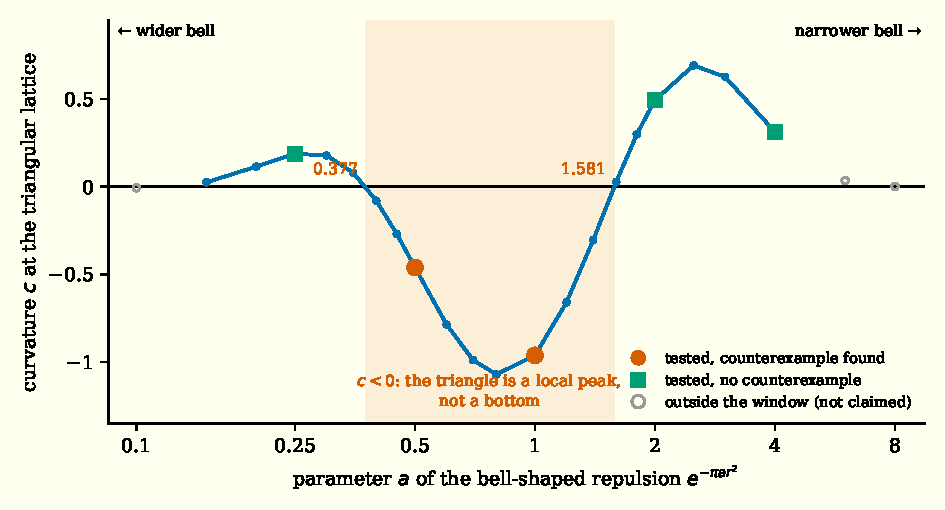
\includegraphics[width=\linewidth]{figures/c12_courbure_largeur}
\caption{Curvature of the zero-point energy at the triangle as a function of the width of the bell: negative (shaded zone) for $0.377<a<1.581$ (below $a\approx0.12$ the curvature is tiny and is not used); floating-point computation (level~X).}
\end{figure}
